% !TEX encoding = UTF-8
% !TEX TS-program = pdflatex
% !TEX root = ../tesi.tex

%**************************************************************
\chapter{L'azienda}
\label{cap:azienda}
%**************************************************************
\section{Introduzione}
Wavelop è un'azienda giovane e innovativa, con sede operativa a Treviso e sede legale a Venezia, che si occupa dello \
sviluppo di applicazioni web e \emph{mobile} per \emph{startup} e imprese. L'ambiente è informale e dinamico, con un focus \
alla flessibilità e al lavoro da remoto. L'azienda riesce a soddisfare le richieste dei clienti grazie all'utilizzo della metodologia Agile \emph{Scrum} ed \
alla creazione di \emph{design user-centered}, realizzando \emph{\gls{mock-up}} e prototipi per ottenere i risultati più adatti. \
Vengono, inoltre, utilizzate le migliori tecnologie in base al progetto richiesto. Ciao

%**************************************************************
\section{Processi aziendali}

\subsection{Metodologia Agile}
La metodologia Agile è un approccio iterativo al \emph{project management} che consente ai \emph{team} di sviluppo \
di consegnare al cliente il prodotto più rapidamente. Ci sono molteplici metodologie che fanno riferimento al \emph{"Agile Manifesto"}, la più diffusa e utilizzata \
dall'azienda, è lo \emph{Scrum}. \
È stato scelto questo \emph{framework} come metodologia di lavoro perché incoraggia i membri del \emph{team} a lavorare insieme ma anche perché si basa sul principio \
dell'apprendimento continuo e sull'adattamento a situazioni che cambiano continuamente, per questo si adatta perfettamente ad una realtà giovane come Wavelop. \\

La prima attività che viene svolta è l'individuazione delle \emph{user stories}, ognuna delle quali, in azienda, viene strutturata nel seguente modo:
\begin{center}
  \textbf{Come [tipo di utente], voglio [intento], in modo che [beneficio]}
\end{center}

Un esempio reale di \emph{user story} scritta durante il mio \emph{stage} è il seguente: 
\newline
\emph{"Come utente Lago o utente EDI voglio poter visualizzare una lista di allegati di una riga della griglia dell'EDI."} \\

Ad ogni \emph{user story} il redattore aggiunge i \emph{tasks} da eseguire per ottenere il risultato richiesto e, inoltre, stima gli \emph{story points}, ovvero il carico di lavoro \
stimato. Successivamente le \emph{user stories} vengono importate in \emph{GitLab} sotto forma di \emph{issues}, questa lista costituisce il \emph{product backlog}. \
A questo punto il \emph{team} è pronto per iniziare il primo \emph{sprint}. \\

\begin{figure}[!ht]
  \begin{center}
    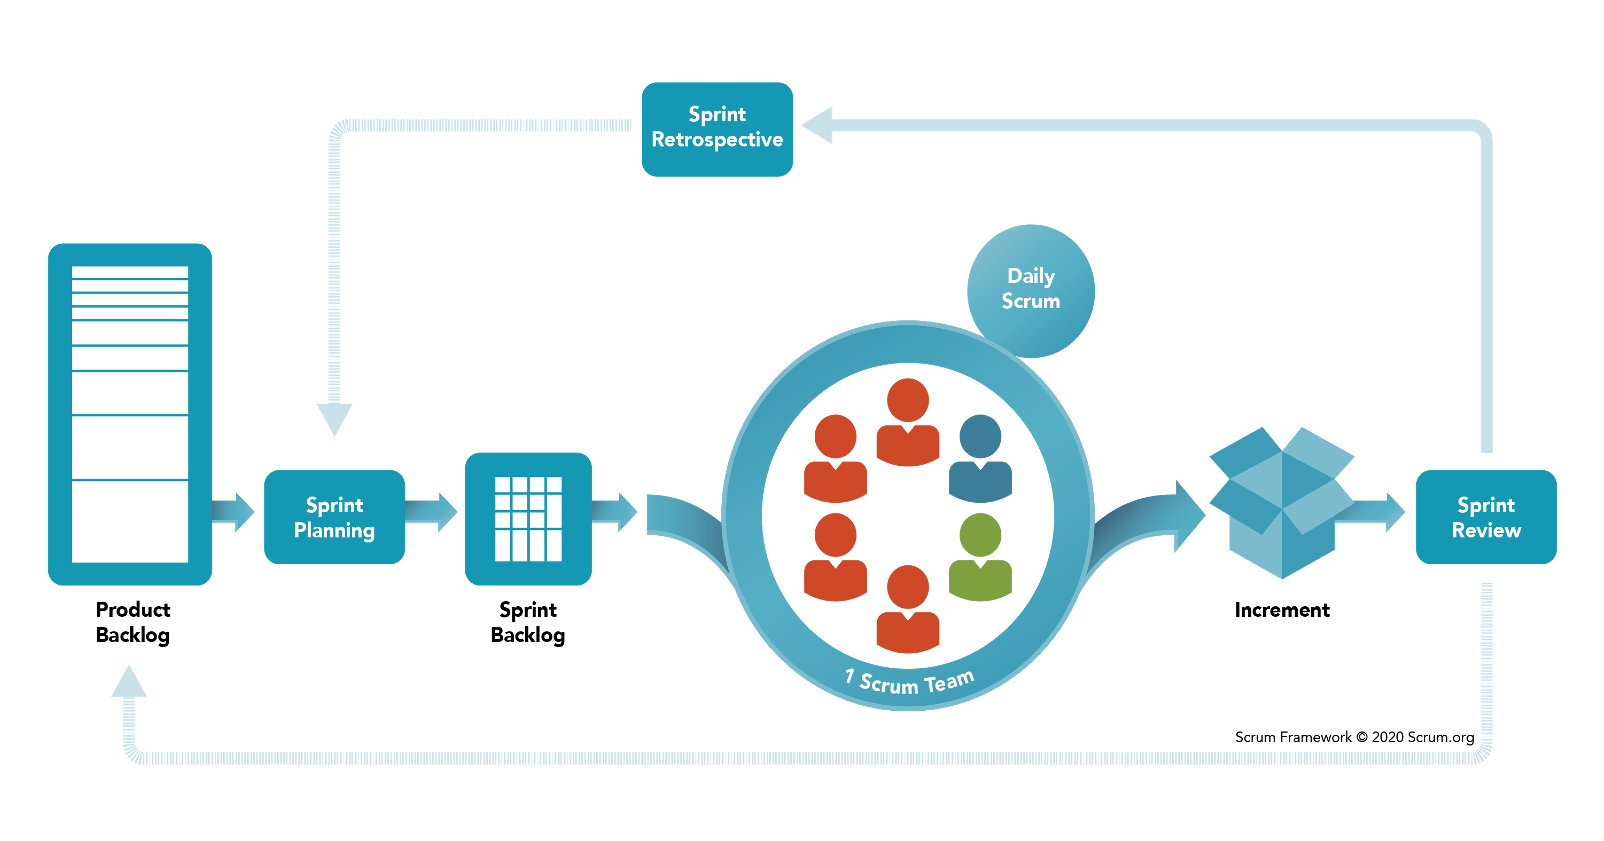
\includegraphics[height=8cm, width=\textwidth]{scrum}
    \caption{Raffigurazione dello Scrum}
    \textbf{Fonte:} \href{https://www.scrum.org}{scrum.org}
  \end{center}
\end{figure}

Prima iniziare uno \emph{sprint}, in Wavelop, il \emph{team} si riunisce per definire l'obiettivo dello \emph{sprint} che si andrà a svolgere, inoltre vengono selezionate \
dal \emph{product backlog} le \emph{user stories} che dovranno essere implementate durante lo \emph{sprint}, andando a costituire lo \emph{sprint backlog}; questa attività \
prende il nome di \emph{Sprint Planning} e, una volta terminata, inizia lo \emph{sprint} vero e proprio. In azienda lo \emph{sprint} dura due settimane, durante le quali il \
\emph{team} implementa le \emph{user stories} presenti nello \emph{sprint backlog}. Durante lo \emph{sprint} ogni mattina, prima di iniziare la giornata lavorativa, viene svolto \
lo \emph{daily scrum meeting}: una breve riunione informale tra i membri del \emph{team}, durante la quale ci si allinea sul lavoro svolto e si pianifica il lavoro della giornata. \
L'azienda ha stabilito che durante questa riunione ogni componente del \emph{team} deve rispondere alle seguenti domande: "Cosa ho fatto ieri?", "Cosa farò oggi?", "Ho avuto qualche problema?"; \
inoltre, adottando molto frequentemente il \emph{remote working} la riunione viene svolta sul \emph{server \textbf{Discord}} dell'azienda. Al termine di ogni \
\emph{sprint}, si svolge una riunione informale tra il \emph{team} e gli \emph{\glspl{stakeholder}} per mostrare il lavoro svolto e per ottenere dei \emph{feedbacks} (\emph{Sprint \
Review}). Sulla base dei \emph{feedbacks} ottenuti durante la \emph{Sprint Review} il capo di progetto decide se rilasciare l'incremento oppure no. Successivamente il \emph{team} \
svolge un'altra riunione per discutere su cosa migliorare nel prossimo \emph{sprint} e su cosa ha funzionato nello \emph{sprint} appena concluso, l'attività viene denominata \emph{Sprint Retrospective}. \
In Wavelop, durante la \emph{Sprint Retrospective}, viene inoltre creato un foglio di calcolo dove vengono inseriti i valori relative a tutte le \emph{user stories} implementate: in particolare \
si valuta la bontà della pianificazione di ogni \emph{user story}. Questo è reso possibile grazie al rendiconto delle ore per ogni singola \emph{issue}, questo valore viene inserito nel foglio di calcolo \
e viene calcolato il valore equivalent in \emph{story points}; successivamente, il \emph{software} effettua il confronto con il valore pianificato in precedenza. In base all'esito del confronto il \emph{team} \
può capire se ha svolto una buona pianificazione o meno.

\subsection{Sviluppo}
Durante la mia permanenza presso l'azienda ho assistito e partecipato al processo di sviluppo, progettando l'architettura del prodotto e implementandola seguendo i principi del \
\emph{\acrfull{tdd}}. Per realizzare un prodotto di buona qualità è fondamentale mantenere il lavoro ben organizzato, per questo motivo è stato definito un \
\emph{workflow} da seguire per la gestione delle \emph{issues}. \\

Quando una \emph{issue} viene presa in carico, per prima cosa, viene assegnato lo stato \emph{"Doing"}, viene specificato lo sviluppatore a cui essa è assegnata e, se non è già presente, \
viene assegnata la \emph{milestone} dello \emph{sprint} corrente. Prima di iniziarne l'implementazione si devono creare una \emph{merge request} e un \emph{feature branch}, solo dopo \
si può procedere all'implementazione vera e propria. Una volta completata l'implementazione, lo sviluppatore modifica lo stato della \emph{issue} in \emph{"To Review"} e assegna la \
\emph{merge rerquest} a una delle due persone designate dall'azienda. \
Solo in caso di esito positivo si procede con l'aggiunta dei cambiamenti al \emph{branch develop} e la chiusura della \emph{issue} assegnandole lo stato \emph{"Closed"}. \\

L'implementazione segue il \emph{\acrlong{tdd}}, ovvero: per prima cosa si scrive un \emph{test}, si esegue il \
\emph{test}, se fallisce si procede a scrivere il codice necessario per farlo passare; vengono svolte queste operazioni fino a quando il \emph{test} non ha successo. \
Successivamente, si eseguono tutti i \emph{test} e solo se tutti hanno successo, se necessario, si procede con il \emph{refactoring}. Nel caso qualche \emph{test} fallisca viene \
scritto il codice per farli passare; tutte queste attività, in azienda, vengono svolte utilizzando il \emph{framework} di \emph{testing \textbf{Jest}} che, oltre a fornire le primitive per scrivere i \emph{tests}, \
può calcolare i dati di \emph{code coverage} consentendo al \emph{team} di valutare la qualità del codice prodotto. La porzione di codice sottostante è un esempio \emph{test} scritto durante lo sviluppo aderendo al \acrshort{tdd}.

\begin{lstlisting}[caption=Esempio di \emph{test}, captionpos=b]
  describe("Testing SupplierService", () => {
    const repo = new SupplierRepository();

    beforeAll(async () => {
      await repo.deleteAll();
      await repo.insert({
        name: "Primo fornitore",
        code: "123456789",
        columns: []
      });
      return 
    })

    it("Get all suppliers should success", async () => {
      const service = new SupplierService(repo);
      const result = await service.findAll();

      return expect(result.length).toBe(1);
    })
  })
\end{lstlisting}

% \begin{figure}[!ht]
%   \begin{center}
%     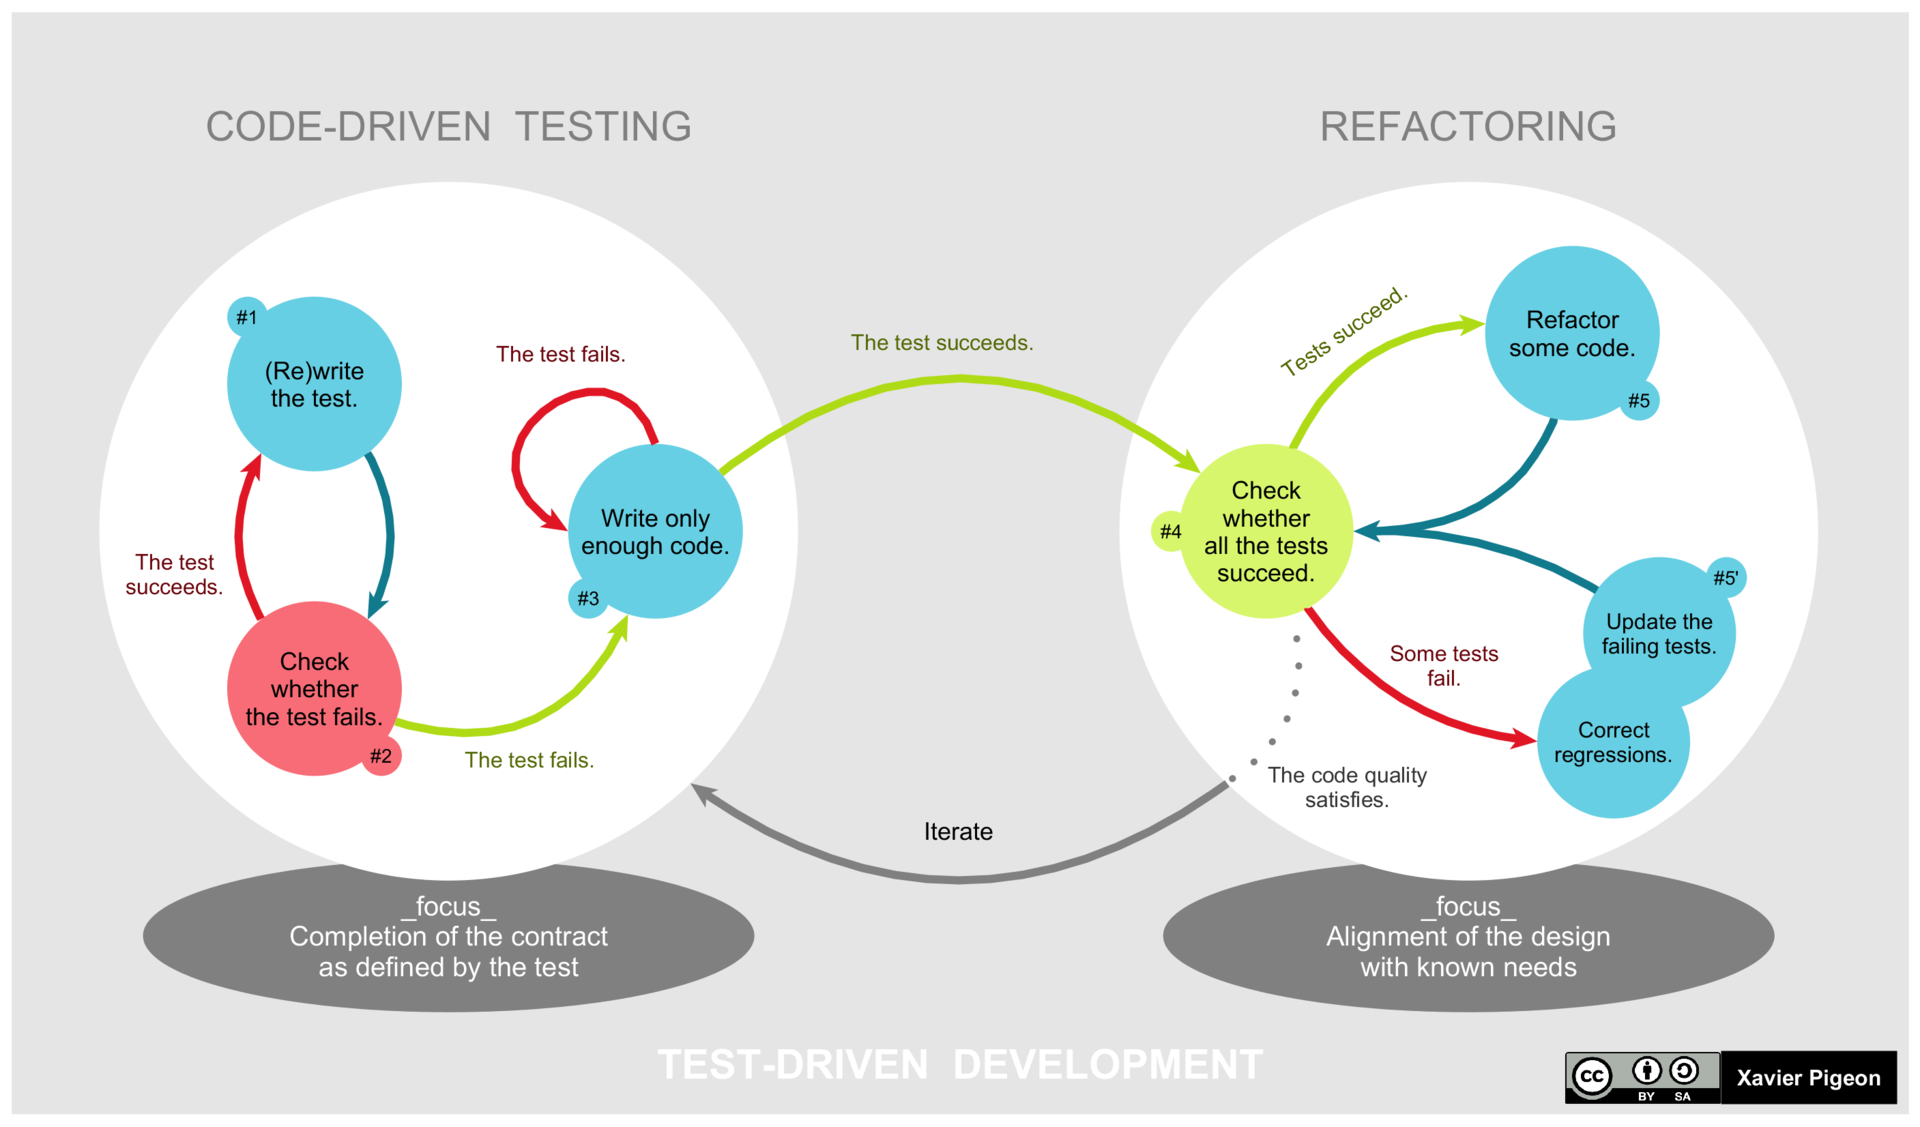
\includegraphics[height=8cm, width=13cm]{tdd-cycle}
%     \caption{\emph{Test-Driven Development cycle}}
%     \textbf{Fonte:} \href{https://www.wikipedia.org}{wikipedia.org}
%   \end{center}
% \end{figure}

%**************************************************************
\section{Strumenti a supporto dei processi}

\subsection{\emph{Git} \& \emph{Gitflow Workflow}}
\emph{Git} è un \emph{Distributed Version Control System}, \emph{open-source} e gratuito, progettato per gestire progetti di grandi e piccole dimensioni con efficienza. \
Facendo uso di \emph{way of working} basato su rilasci programmati, l'azienda ha deciso di utilizzare il modello \emph{Gitflow Workflow}. \
Ogni progetto è costituito da cinque tipi di \emph{branch} diversi: \textbf{\emph{main}}, \textbf{\emph{develop}}, \textbf{\emph{release}}, \textbf{\emph{hotfix}} e \
\textbf{\emph{feature}}. I \emph{branches} di base, che saranno sempre presenti nel ciclo di vita del progetto sono:
\begin{itemize}
  \item \emph{main} nel quale si trova lo storico delle versioni rilasciate in produzione dall'azienda;
  \item \emph{develop} nel quale troviamo lo storico completo del progetto. 
\end{itemize}  

I seguenti tipi di \emph{branch}, a differenza dei precedenti, hanno vita limitata: \
\begin{itemize}
  \item i \emph{branch} di tipo \emph{feature} sono adibiti allo sviluppo di nuove funzionalità, al termine del quale viene incorporato nel \emph{branch develop}; 
  \item i \emph{branch} di tipo \emph{release} vengono utilizzati per cominciare un nuovo ciclo di rilascio per una nuova versione, al termine del quale viene incorporato nel \
  \emph{branch main}; 
  \item i \emph{branch} di tipo \emph{hotfix} sono adibiti alla correzione di piccoli \emph{bug} in produzione, una volta risolto il problema viene incorporato nel \emph{branch main}.
\end{itemize}

\vspace{10pt}
  \begin{figure}[!ht]
    \begin{center}
      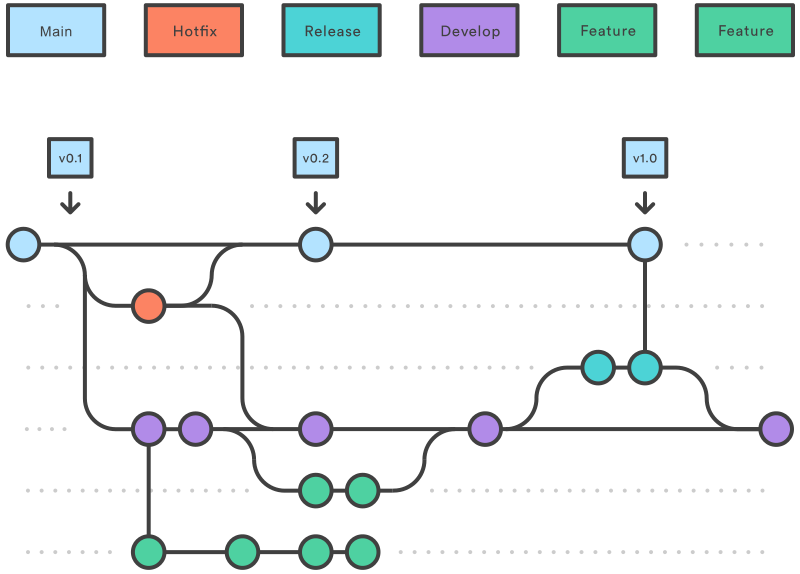
\includegraphics[height=8cm, width=12cm]{gitflow-workflow}
      \caption{Gitflow Workflow}
      \textbf{Fonte:} \href{https://www.atlassian.com}{atlassian.com}
    \end{center}
  \end{figure}
\vspace{10pt} 

\subsection{\emph{GitLab}}
GitLab, a differenza di git, è una piattaforma di \emph{hosting} per \emph{git repositories}; inoltre offre diversi servizi \
per la gestione del progetto, tra i quali:

\begin{itemize}
  \item \emph{Issue Tracking System};
  \item \emph{Project Board};
  \item \emph{Merge Requests}.
\end{itemize}

\subsubsection{\emph{Issue}}
In \emph{GitLab} le \emph{issues} rappresentano i \emph{tasks} da implementare ai fini dell'avanzamento in un progetto. Nel contesto lavorativo di Wavelop, le \emph{issues}, \
sono le \emph{user stories} e sono caratterizzate da: un titolo, una descrizione e uno o più utenti che ce l'hanno in carico; inoltre, viene aggiunta una \
\emph{milestone} (lo \emph{sprint} a cui è assegnata), delle \emph{labels} ai fini di una migliore organizzazione e, infine, vengono aggiunti gli \emph{story points} che forniscono \
una stima del tempo che verrà impiegato per implementarla. L'insieme di tutte le \emph{issues} costituisce il \emph{product backlog} mentre, le \emph{issues} \
appartenenti ad una determinata \emph{milestone} costituiscono lo \emph{sprint backlog}.
\begin{figure}[!ht]
  \begin{center}
    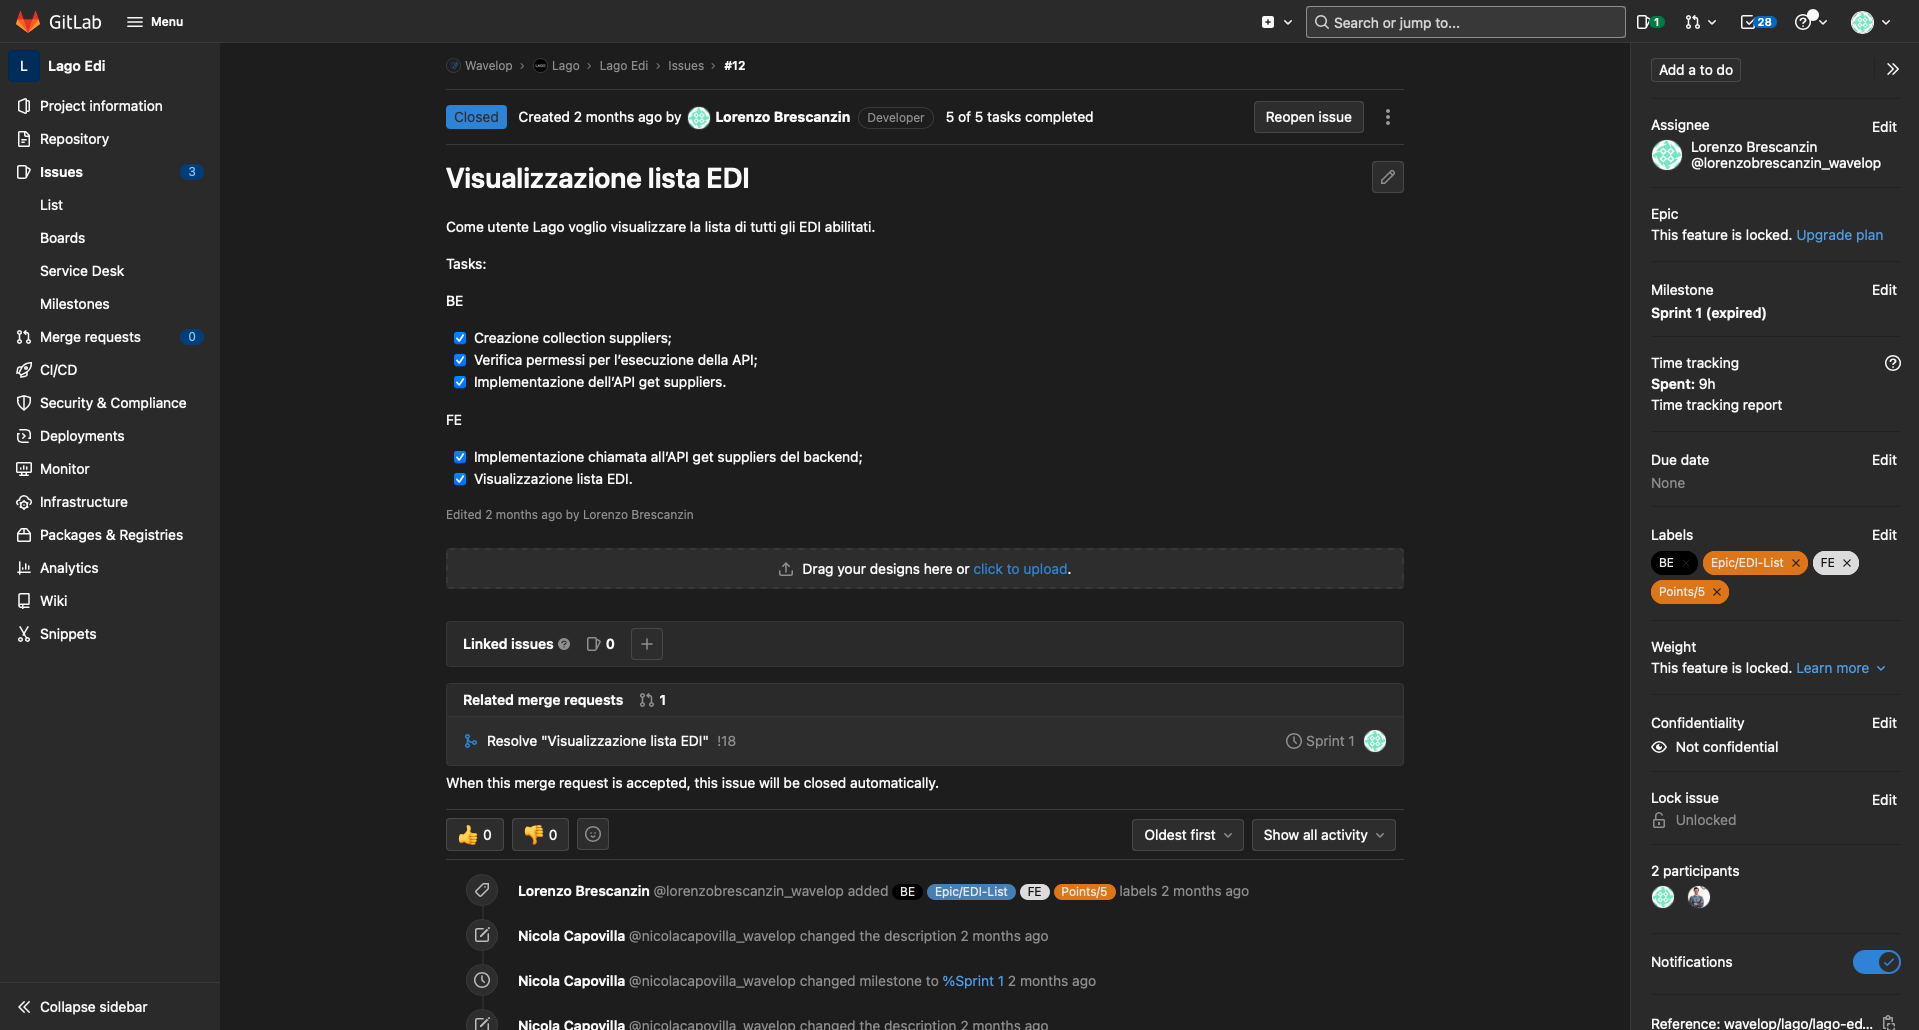
\includegraphics[height=8cm, width=13cm]{issue}
    \caption{Esempio di una \emph{issue}}
  \end{center}
\end{figure}

\subsubsection{\emph{Project Board}}
Una \emph{project board} è un raccoglitore di \emph{issues}, organizzate in colonne, utilizzato per una migliore organizzazione del lavoro e per facilitare \
la verifica dello stato di avanzamento del progetto. In Wavelop la \emph{project board} è costituita da quattro colonne che indicano lo stato in cui si trova una \emph{issue}:

\begin{itemize}
  \item \textbf{\emph{Open}:} la \emph{issue} deve ancora essere presa in carico e quindi deve ancora essere implementata;
  \item \textbf{\emph{Doing}:} la \emph{issue} è stata presa in carico da un componente del \emph{team} ed è in implementazione;
  \item \textbf{\emph{To Review}:} la \emph{issue} è stata implementata ed è pronta per la revisione da parte del \emph{reviewer}. Sulla base dell'esito di questa attività \
  la \emph{issue} viene spostata in \emph{Doing}, nel caso di esito negativo, o in \emph{Closed}, in caso di esito positivo;
  \item \textbf{\emph{Closed}:} la \emph{issue} è stata completata e viene aggiunta al \emph{branch develop}.
\end{itemize}

\begin{figure}[!ht]
  \begin{center}
    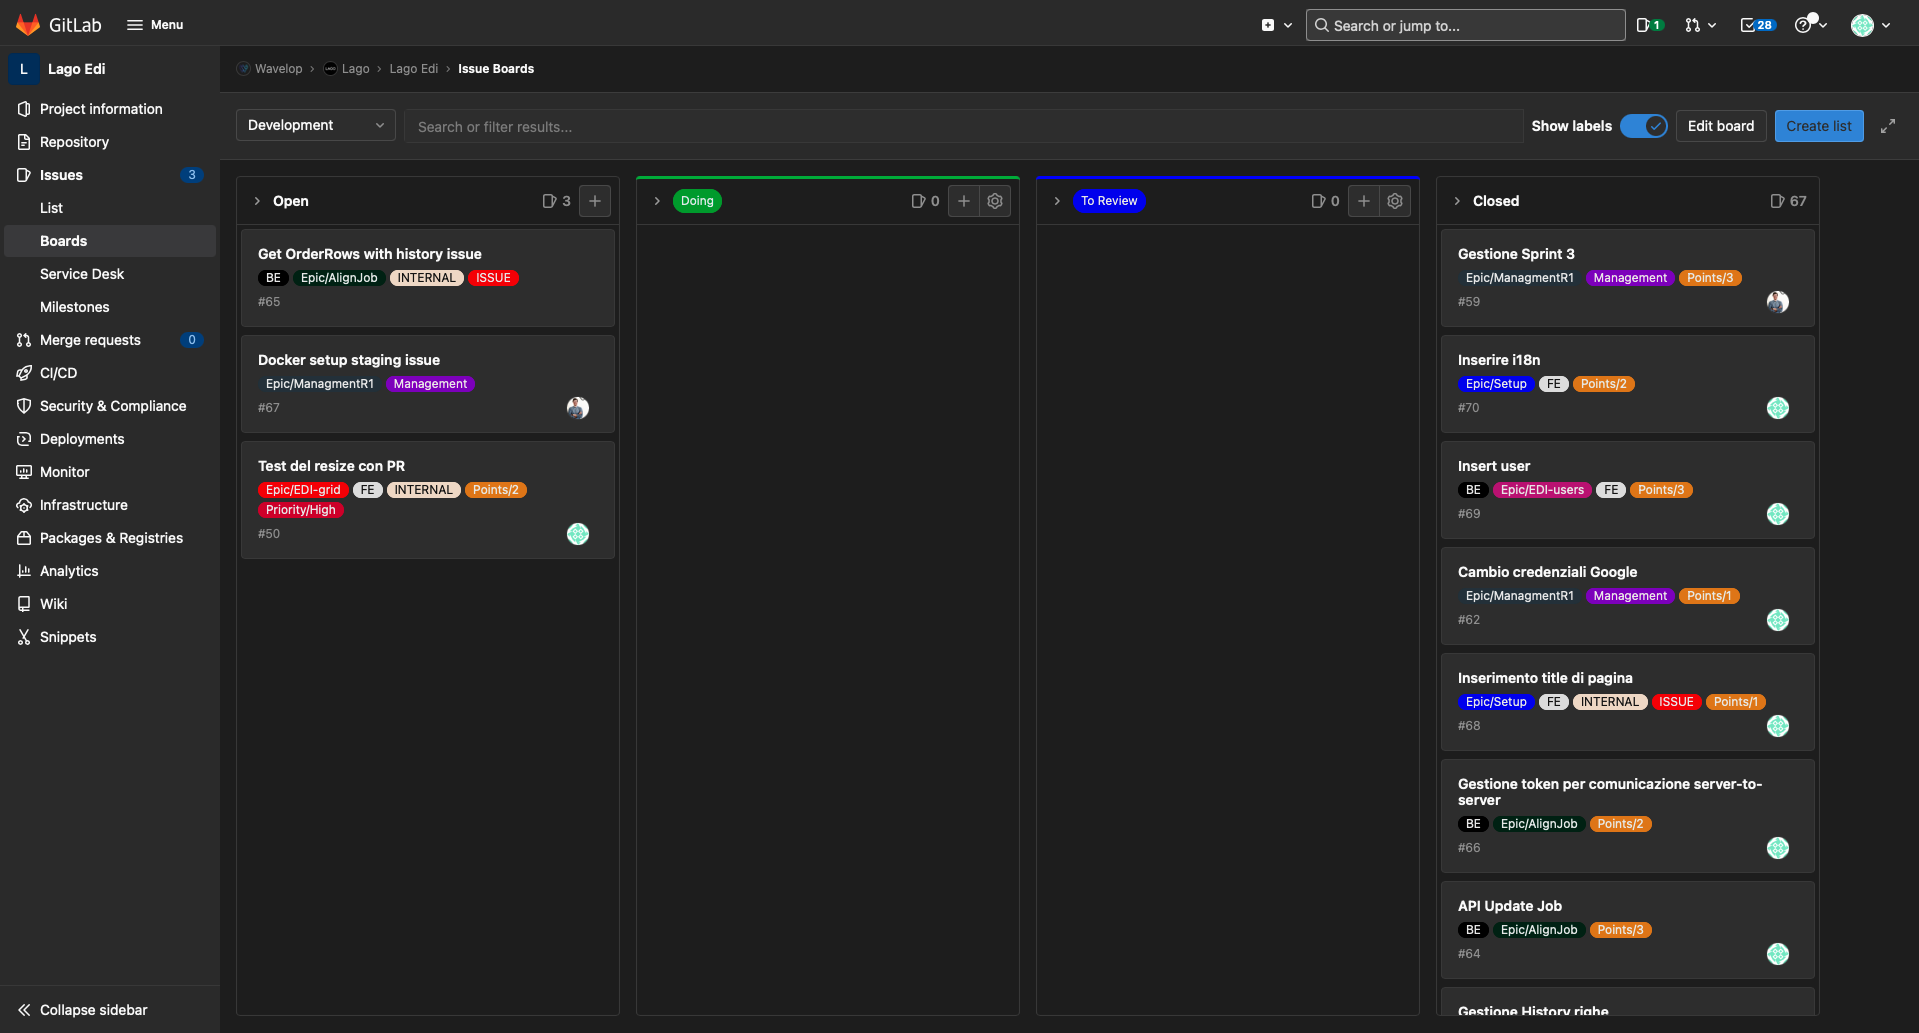
\includegraphics[height=8cm, width=13cm]{project-board}
    \caption{Esempio di \emph{project board}}
  \end{center}
\end{figure}

\subsubsection{\emph{Merge Requests}}
Le \emph{merge requests} vengono utilizzate per tracciare e revisionare i cambiamenti prima che essi vengano incorporati nei \emph{branch main} o \emph{develop}. All'interno del \
\emph{way of working} di Wavelop, vengono utilizzate anche per discutere di ciò che è stato implementato e di modifiche da apportare. Quando si prende in carico una \emph{issue}, si \
crea una \emph{merge request} e un \emph{feature branch}; una volta che il \emph{reviewer} ha approvato i cambiamenti implementati, il \emph{feature branch} viene unito al contenuto \
del \emph{branch develop} e successivamente eliminato.

\begin{figure}[!ht]
  \begin{center}
    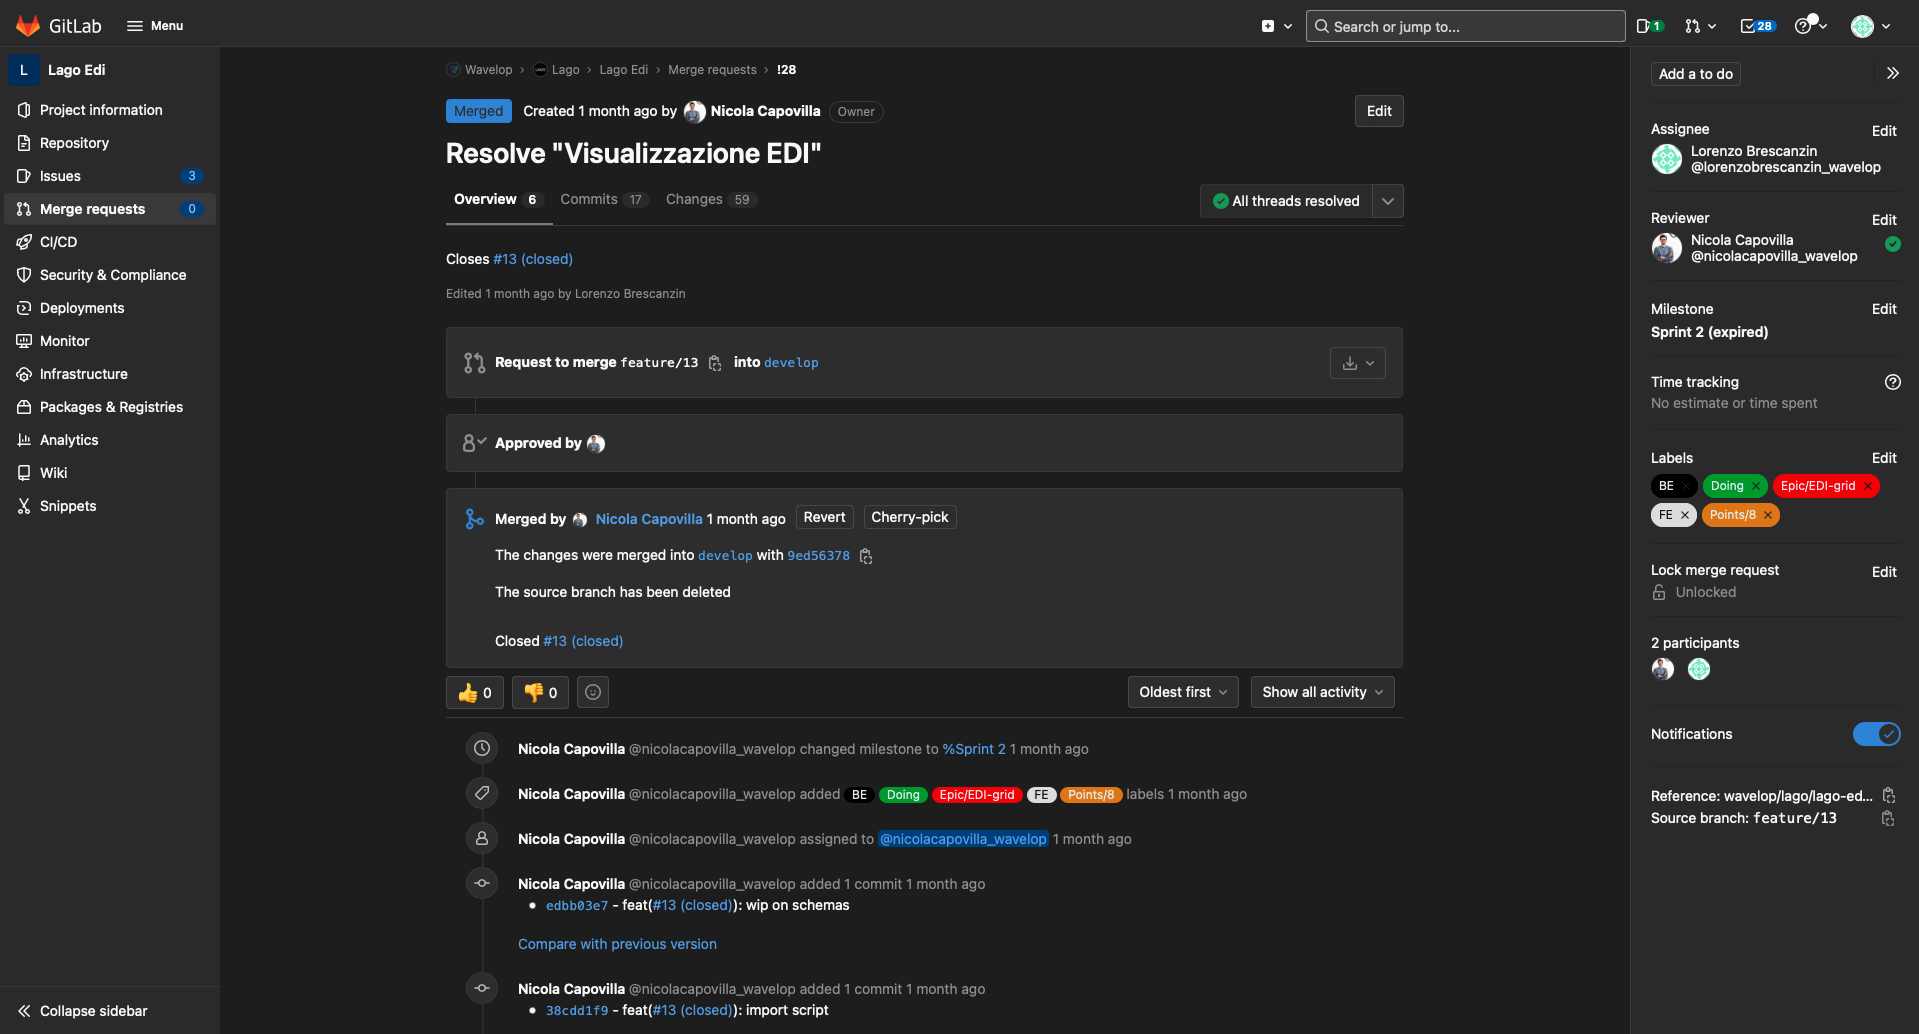
\includegraphics[height=8cm, width=13cm]{merge-request}
    \caption{Esempio di \emph{merge request}}
  \end{center}
\end{figure}

\newpage
\subsection{\emph{Google Workspace}}
\emph{Google Workspace} è un insieme di strumenti di collaborazione e produttività sviluppato da Google. \
I servizi utilizzati maggiormente dall'azienda sono:

\begin{itemize}
  \item \emph{Gmail} per le comunicazioni formali con clienti e \emph{team};
  \item \emph{Calendar} per la gestione degli impegni aziendali;
  \item \emph{Drive} per la memorizzazione di file nel \emph{cloud};
  \item \emph{Meet} per le riunioni formali con i clienti;
  \item \emph{Google Docs Suite} per la redazione della documentazione e per la realizzazione delle presentazioni per i clienti.
\end{itemize}

%**************************************************************
\section{Rapporto con l'innovazione}
L'azienda è in costante aggiornamento sulle nuove tecnologie partecipando ad incontri tecnologici con relatori di spicco: \emph{Google} e \emph{Amazon}, \
per citarne alcuni; in generale, è molto propensa all'innovazione accettando la presa in carico di progetti innovativi che sfruttano \
i moderni \emph{smart speakers}, l'architettura \emph{Serverless} o nell'ambito dell'\acrfull{iot}. Un altro aspetto in cui Wavelop può essere definita innovativa è l'adozione \
del \emph{remote working} sin dagli albori: questa scelta ha permesso ad ogni dipendente di lavorare nelle condizioni in cui performa al meglio, portando benefici non solo al \
fatturato dell'azienda ma anche alla persona stessa. Grazie all'esperienza maturata nel lavoro da remoto, l'azienda è riuscita a non subire direttamente gli effetti dovuti \
alla pandemia. Un altro aspetto importante è la costante ricerca di giovani da formare con il \emph{focus} sull'innovazione garantendo così un futuro alla visione aziendale.